\documentclass[11pt]{article}
\usepackage[a4paper, margin=2.5cm]{geometry}
\usepackage[slovene]{babel}
\usepackage[utf8]{inputenc}
\usepackage[T1]{fontenc}
\usepackage{amsthm}
\usepackage{amsmath}
\usepackage{cite}
\usepackage{graphicx}

% Definicija ukazov
\newcommand{\f}{\mathcal{F}}
\newcommand{\RR}{\mathbb{R}}  % Realna števila

\theoremstyle{definition}
\newtheorem{definicija}{Definicija}

\theoremstyle{plain}
\newtheorem{izrek}{Izrek}

\title{Brownovo gibanje}
\author{Matej Rojec}
\date{}

\begin{document}

\maketitle 

Brownovo gibanje (več v \cite{karatzas1991brownian}) je intuitivno slučajen proces, % Sklic na knjigo
ki predstavlja naključno gibanje delcev v mediju.
    
    % Slika: PerrinPlot2.pdf
    % Napis pod sliko: 
    % Reprodukcija slike iz Jean Baptiste Perrin, \emph{Mouvement brownien et réalité moléculaire}, Ann. de Chimie et de Physique (VIII) 18, 5-114, 1909
\begin{figure}
    \centering
    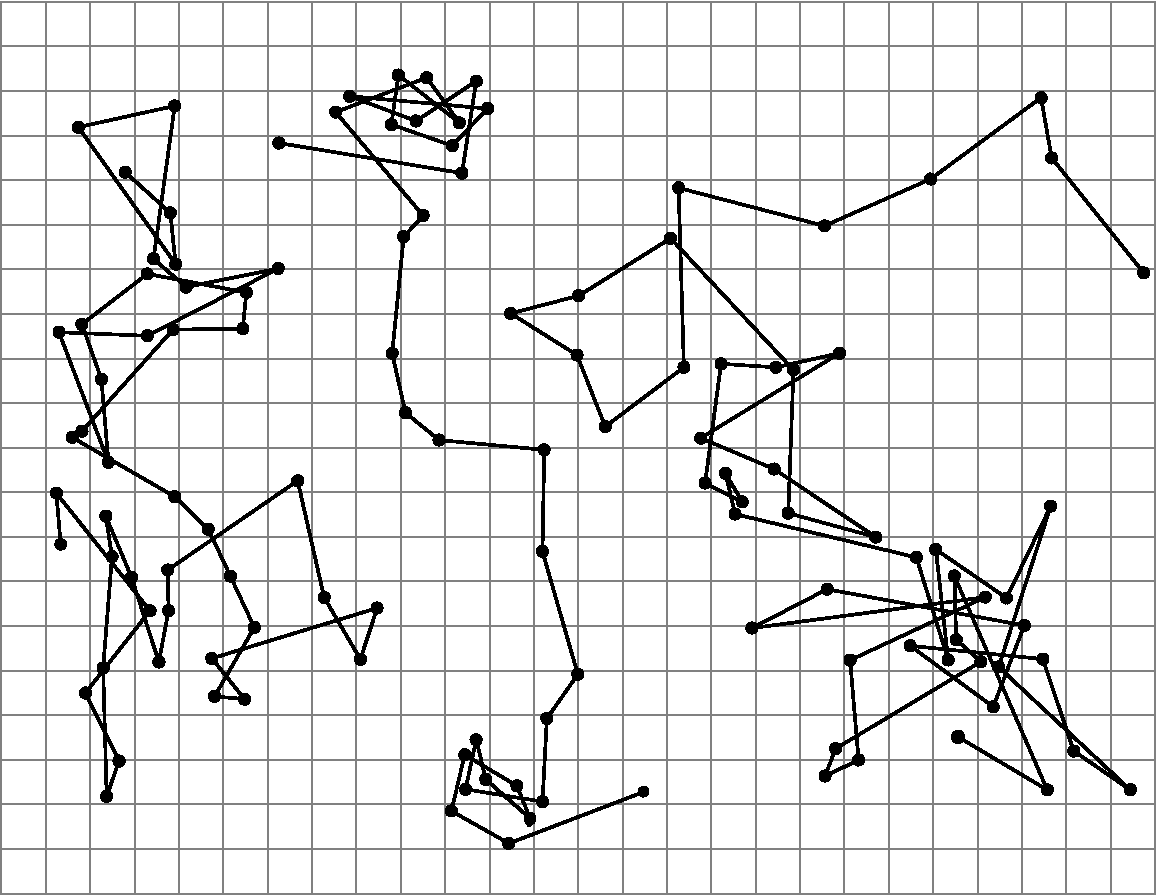
\includegraphics[width=0.5\textwidth]{PerrinPlot2.pdf}
    \caption{Reprodukcija slike iz Jean Baptiste Perrin, \emph{Mouvement brownien et réalité moléculaire}, Ann. de Chimie et de Physique (VIII) 18, 5-114, 1909}
    \label{fig:perrin_plot}
\end{figure}

    % Začetek definicije
    \begin{definicija}
        \begin{itemize}
            \item Standardno Brownovo gibanje $\{B_t\}_{t \geq 0}$ je slučajen proces z naslednjimi lastnostmi: 
        $B_0 = 0$.
            \item Prirastki $B_{t_n} - B_{t_{n-1}}, B_{t_{n-1}} - B_{t_{n-2}}, \ldots, B_2 - B_1, B_1 - B_0$ so neodvisne slučajne spremenljivke, za vsak $t_0 \leq t_1 \leq \cdots \leq t_{n-1} \leq t_n$.
            \item Za vsak $t \geq 0$ in $h > 0$ velja $B_{t+h} - B_t \sim \mathcal{N}(0, h)$.
            \item Funkcija $t \mapsto B_t$ je zvezna skoraj gotovo. 
        \end{itemize}  
    \end{definicija}
    % Konec definicije
    
    Preden zapišemo izrek, definirajmo še pojem časa ustavljanja.
    
    % Začetek definicije
    \begin{definicija}
        Slučajna spremenljivka $\tau$ na verjetnostnem prostoru $(\Omega, \mathcal{F}, P)$ z vrednostmi v \(\mathbb{R}^+\) je čas ustavljanja glede na filtracijo $(\mathcal{F}_t)_{t \geq 0}$, če velja: 
        \[
        \forall t \geq 0 : \lbrace \tau \leq t \rbrace \in \mathcal{F}_t.
        \]
    \end{definicija}
% Konec definicije
    
    Zdaj lahko zapišemo izrek \ref{thm:stopped_brownian}. % Sklic na izrek z oznako thm:stopped_brownian
    
    % Začetek izreka
    \begin{izrek}
    \label{thm:stopped_brownian}  
    Naj bo $\{B_t\}_{t \geq 0}$ (standardno) Brownovo gibanje, $\tau$ čas ustavljanja glede na 
    $(\mathcal{F}_t)_t \geq 0$ in naj bo $P [\tau < \infty] = 1$.
    Potem je tudi proces:
    \[
    \hat{B} := \{B_{T+t} - B_T \mid t \geq 0\}
    \]
    (standardno) Brownovo gibanje in neodvisen od $\mathcal{F}_T$.
    \end{izrek} 
    % Konec izreka
    
    % bibliografija
    \bibliographystyle{plain}
    \bibliography{knjiga}

\end{document}